\subsection{Suppressing quantum errors by scaling a surface code logical qubit}

Scaling of the surface code is essential to building large-scale quantum computers. Google Quantum AI has demonstrated successful implementation of the scaling of surface code, showing that increasing the number of qubits can indeed improve the performance of a logical qubit, suppressing the error rate while also dealing with additional problems associated with scaling.

The research team of Google Quantum AI implemented a distance-5 surface code using 72 qubits. By comparing it to a smaller distance-3 code, they observed a reduction in logical error rates per cycle, from 3.028\% to 2.914\%.

This work shows that quantum error correction improves with scaling, essential for developing large quantum systems for applications in cryptography, optimization, and simulations beyond classical capabilities. Using a 72-qubit device, the team showed that larger codes can outperform smaller ones, highlighting the potential of scaling for better quantum error correction. This is a key step towards making quantum computing viable for complex computations.



\begin{figure}[h]
    \centering
    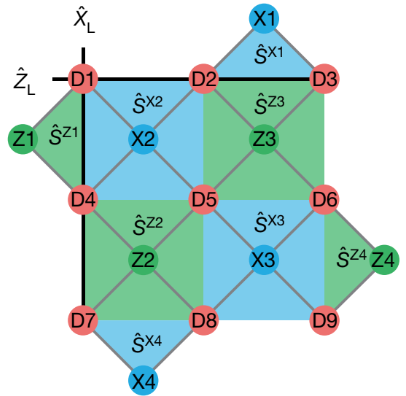
\includegraphics[width=0.4\textwidth]{sections/5_practical_implementation/representation.png}
    \caption{}
\end{figure}

\subsection{Realizing repeated quantum error correction in a distance-three surface code}
Successful implementation of the surface code is a milestone in quantum error correction, showing that practical realization is possible, we are one step closer to making a large-scale quantum computer. Using 17 physical qubits in a superconducting circuit, researchers have encoded quantum information in a distance-three logical qubit. In a correction cycle of 1.1 microseconds that can correct both bit-flip and phase-flip errors, they have successfully preserved the cardinal states of the qubit. By repeatedly correcting errors, a low error rate of 3\% per cycle shows that the surface code does suppress the error probability as theory suggests. This breakthrough brings us closer to large quantum computing systems that can perform computation out of reach of the capacities of modern classical computers.

This achievement demonstrates the robustness of the surface code in a practical setup, supporting its potential for fault-tolerant quantum computing. By achieving low error rates and preserving qubit states, the experiment validates theoretical predictions and advances the development of scalable quantum computers.
